%!TEX root = origin.TEX
\chapter{Desarrollo de la Investigación}
\pagenumbering{arabic}
\setcounter{page}{20}
\renewcommand{\baselinestretch}{2} %doble espacio paratodo el texto

\section{Análisis del conjunto de imágenes}

\subsection{Colección de Señales de Tránsito de Alemania}

\subsubsection{Datos para el entrenamiento}

En esta colección consta de un total de 51839 imágenes distribuidas en 43 clases no necesariamente balanceadas con un tamaño de 32 x 32 pixeles.

\begin{figure}[H]
	\begin{center}
	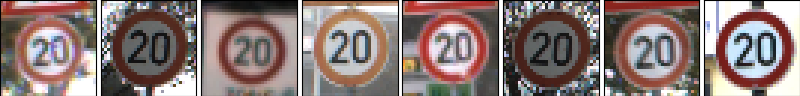
\includegraphics[width=1\textwidth]{images/desarrollo/imagenes/1_(1).png}
	\end{center}
	\begin{center}
	\caption{\small{Señal 20 km}}
	\end{center}
	\vspace{-1.5em}
\end{figure}

\begin{figure}[H]
	\begin{center}
	
\includegraphics[width=1\textwidth]{images/desarrollo/imagenes/1_(2).png}
	\end{center}
	\begin{center}
	\caption{\small{Señal 20 km}}
	\end{center}
	\vspace{-1.5em}
\end{figure}

\begin{figure}[H]
	\begin{center}
	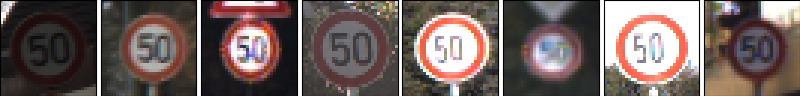
\includegraphics[width=1\textwidth]{images/desarrollo/imagenes/1_(3).png}
	\end{center}
	\begin{center}
	\caption{\small{Señal 20 km}}
	\end{center}
	\vspace{-1.5em}
\end{figure}

\begin{figure}[H]
	\begin{center}
	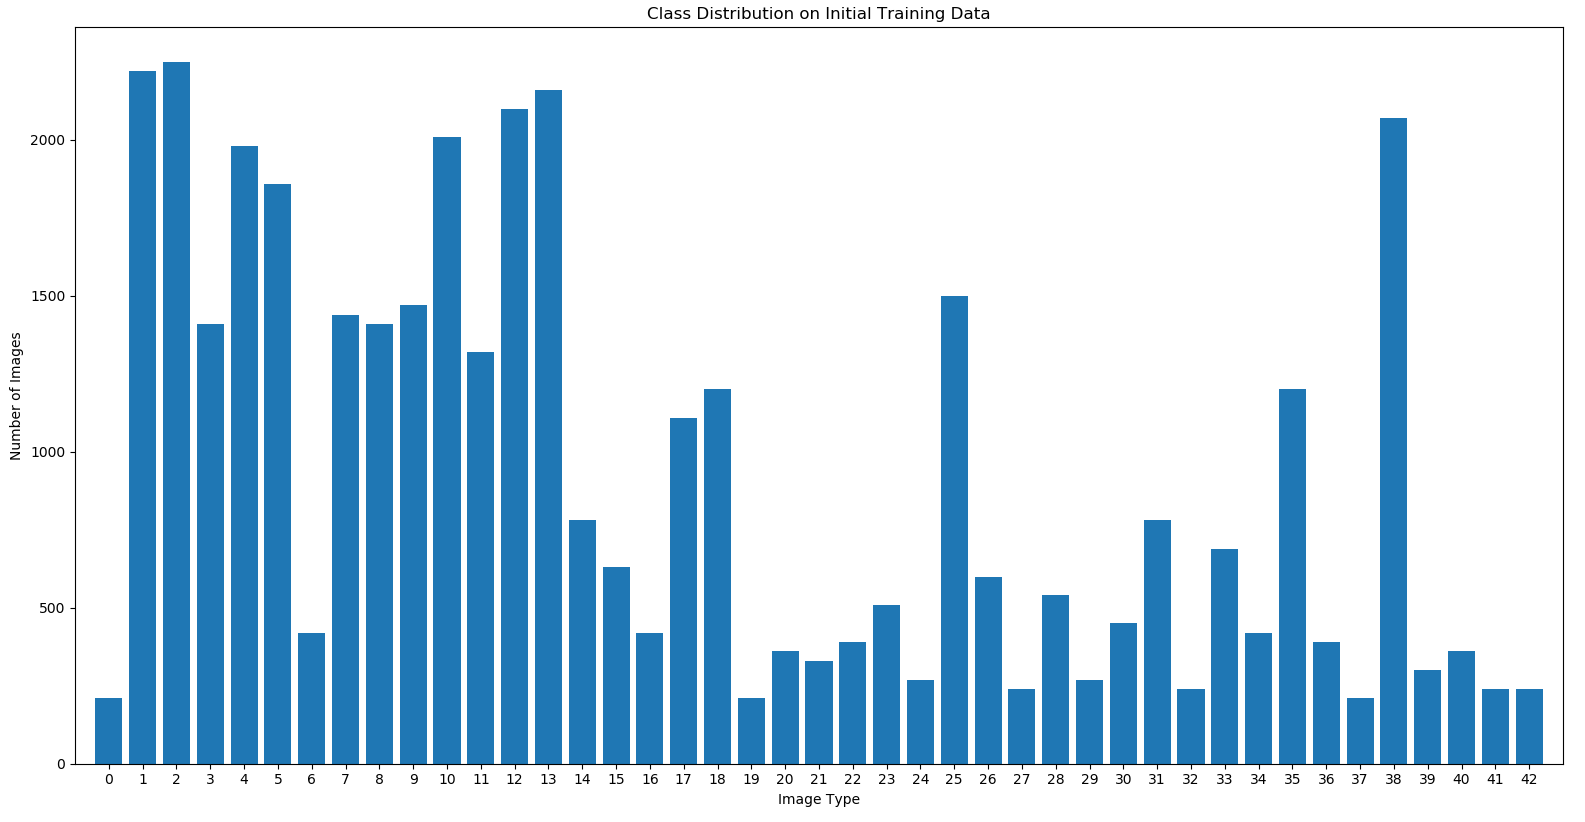
\includegraphics[width=1\textwidth]{images/desarrollo/histograms/initial39209}
	\end{center}
	\begin{center}
	\caption{\small{Distribución de ejemplos por señal para el entrenamiento}}
	{\small{Fuente propia}}
	\end{center}
	\vspace{-1.5em}
\end{figure}



\subsubsection{Datos para la evaluación}
Para la etapa de evaluación se cuenta con un conjunto de 12630 imágenes, de igual manera no necesariamente balanceadas y que no son utilizadas durante el proceso de entrenamiento para obtener resultados confiables a la hora de evaluar el resultado del entrenamiento. 

\begin{figure}[H]
	%\begin{center}
	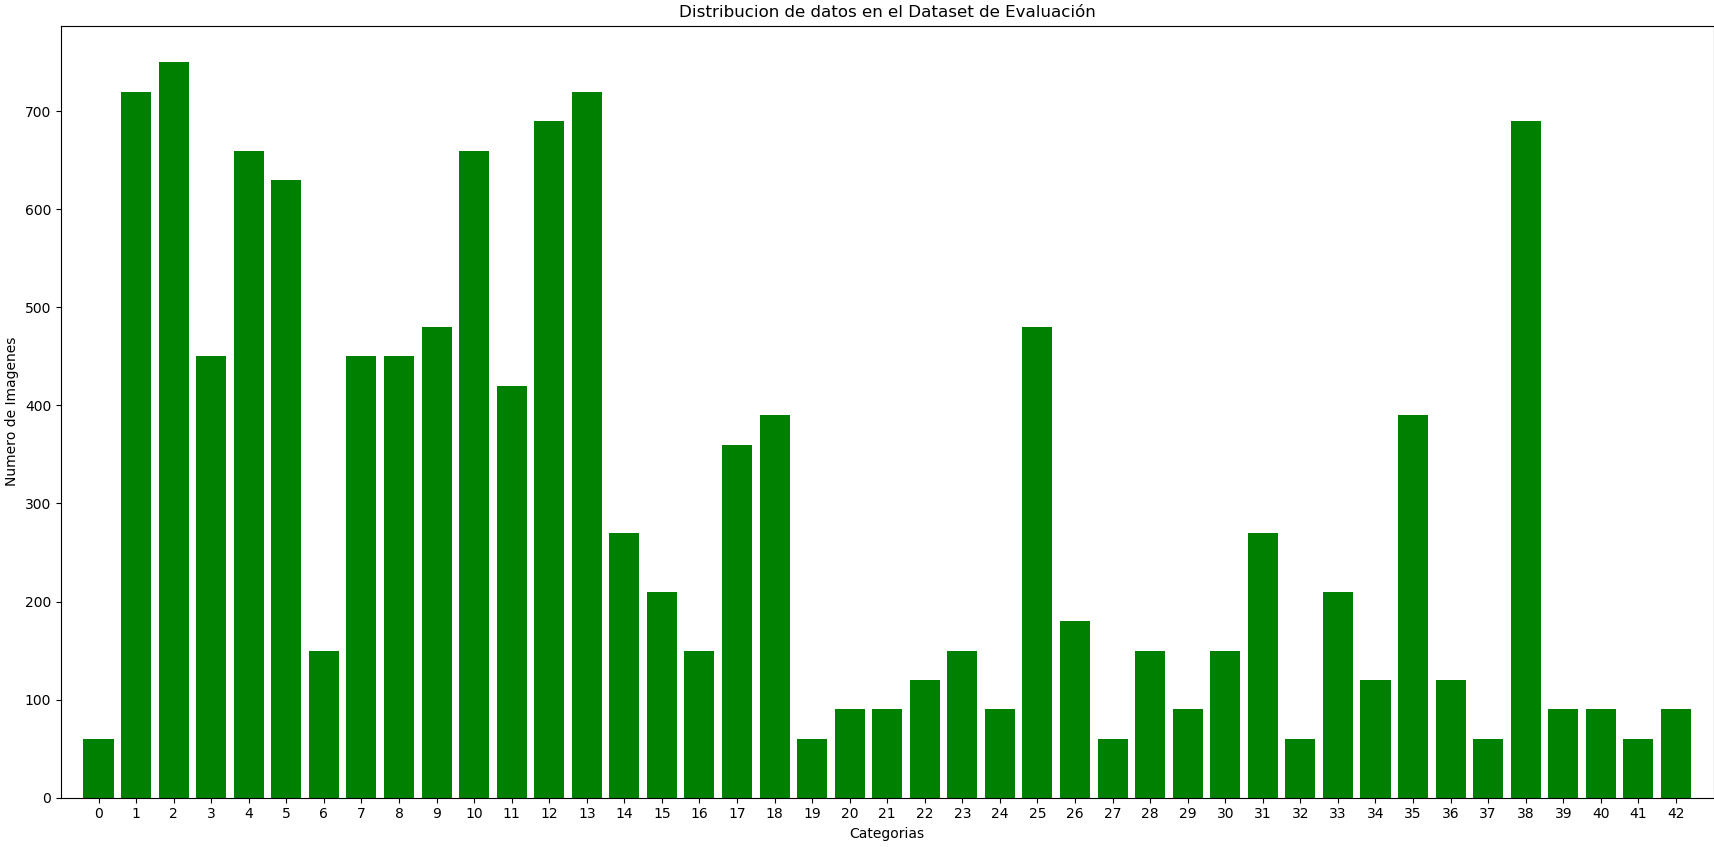
\includegraphics[width=1.1\textwidth]{images/desarrollo/histograms/initialTest12630}
	%\end{center}
	\begin{center}
	\caption{\small{Distribución de ejemplos por señal para la evaluación}}
	{\small{Fuente propia}}
	\end{center}
	\vspace{-1.5em}
\end{figure}

\subsection{Pre-procesamiento de Imágenes(Normalization)}
El pre-procesamiento habitual en este caso consta en escalar los valores de cada píxel entre 0 y 1(ya que actualmente se presentan en el rango de tonalidad entre 0 y 255). Al mirar las imágenes, la ecualización del histograma también puede ser útil. Aplicaremos ecualización de histograma localizado, ya que parece mejorar aún más la extracción de características en nuestro caso.

Como Pierre Sermanet y Yann LeCun mencionaron en su artículo\citep{LeCun}, el uso de canales de color no pareció mejorar mucho las cosas, en esta investigación se usará un solo canal en el modelo, es decir las imágenes estarán en escala de grises en lugar de tener 3 canales de colores.

Para convertir un color de un espacio de color basado en un modelo de color RGB típico de gamma comprimido (no lineal) a una representación en escala de grises de su luminancia, primero se debe eliminar la función de compresión gamma mediante la expansión gamma (linealización) para transformar la imagen en un RGB lineal espacio de color, de modo que la suma ponderada apropiada se puede aplicar a los componentes de color lineales ($R_{linear} , G_{linear} , B_{linear}$) para calcular la luminancia lineal $Y_{linear}$.

Para imágenes en espacios de color como Y'UV y sus derivados, que se usan en sistemas de TV y video a color estándar como PAL, SECAM y NTSC, un componente de luma no lineal ($Y'$) se calcula directamente a partir de intensidades primarias comprimidas con gamma como una suma ponderada, que aunque no es una representación perfecta de la luminancia colorimétrica, puede calcularse más rápidamente sin la expansión gamma y sin la compresión utilizadas en los cálculos fotométricos o colorimétricos,\citep{POYNTON2003257}. En los modelos Y'UV y Y'IQ utilizados por PAL y NTSC, el componente rec601 luma ($Y'$) se calcula como:
$Y' = 0.299R' + 0.587G' + 0.114B'$


..... IMAGENES.....

%\subsection{Proceso de Anotacion de la data}
\subsection{Proceso de Aumento de Datos(Data Augmentation)}

Las redes convolucionales durante el aprendizaje profundo requieren una gran cantidad de datos para conseguir realizar un mejor entrenamiento y obtener un modelo que generalice eficazmente,\citep{DL_augmentData}. Muchas veces esta recopilación de datos suele ser costosa y laboriosa es por eso que el proceso de Data Augmentation ayuda a superar este problema a través del uso de métodos o técnicas de procesamiento de imágenes. En esta investigación son utilizadas las siguientes técnicas:


\begin{figure}[H]
	%\begin{center}
	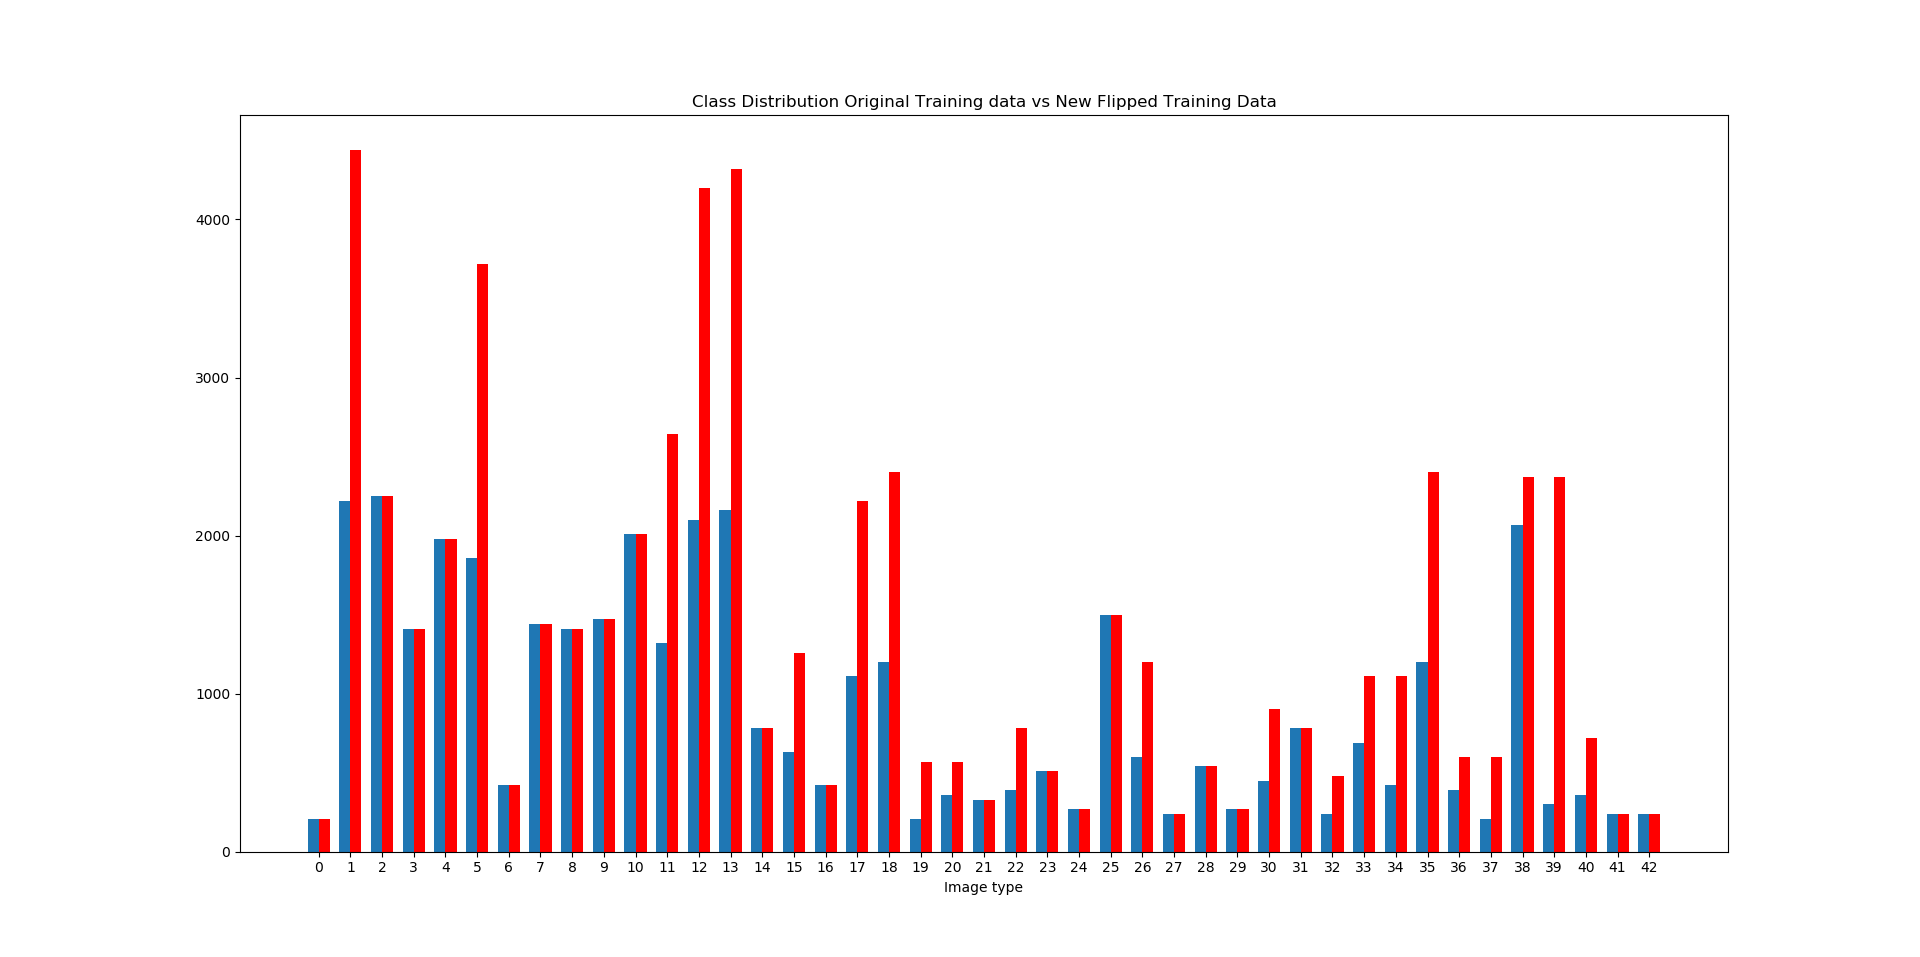
\includegraphics[width=1.1\textwidth]{images/desarrollo/histograms/flippedImg_59698}
	%\end{center}
	\begin{center}
	\caption{\small{Ilustración de un modelo de aprendizaje profundo}}
	{\small{Fuente propia}}
	\end{center}
	\vspace{-1.5em}
\end{figure}